\Aufgabe[Computing the (Greatest) Bisimulation Relation \hfill\textbf{(1 Point)}]

Let $K_1 = (S_1, R_1, L_1)$ and  $K_2 = (S_2, R_2, L_2)$ be two Kripke structures over a set of atomic predicates $\mathit{AP}$.
The relations $H_n \subseteq S_1 \times S_2$ are inductively defined by:
\begin{itemize}
\item $(s_1,s_2) \in H_0$ iff $L_1(s_1) = L_2(s_2)$.
\item $(s_1,s_2) \in H_{n+1}$ iff
    \begin{enumerate}[(i)]
    \item $(s_1,s_2) \in H_n$,\qquad ($\star$)
    \item for all $(s_1,t_1) \in R_1$ there exists a $(s_2,t_2) \in R_2$ with $(t_1,t_2) \in H_n$, and
    \item for all $(s_2,t_2) \in R_2$ there exists a $(s_1,t_1) \in R_1$ with $(t_1,t_2) \in H_n$.
    \end{enumerate}
\end{itemize}

\begin{enumerate}

	\item Compute the sequence $H_0, H_1, H_2,\ldots$ for the Kripke structures $K_1$ and $K_2$ from Exercise 2.
    
	\item Show that the sequence $H_0, H_1, H_2,\ldots$ \emph{stabilizes} for all finite Kripke structures $K_1$ and $K_2$, i.e., there is a $n \ge 0$ such that $H_n = H_{n+1}$.
    
	\item Construct Kripke structures $K_1^n$ and $K_2^n$ such that the sequence $H_0, H_1, H_2,\ldots$ stabilizes after exactly $n$ steps.

\end{enumerate}

a.)

\textbf{Solution:}

\bigskip

Let $K_{1}=(S,R,L_{1})$ and $K_{2}=(S,R,L_{2})$ be two Kripke structures
with the same set of states $S$ and the same transition relation $R$ such
that $L_{1}(s)\subseteq L_{2}(s),\Forall s\in S$.\medskip

Let $H^{\ast }$ be the \textit{largest possible bisimulation} between the
structures $K_{1}$ and $K_{2}$ with $S=S_{1}=S_{2}$ and $R=R_{1}=R_{2}$.

Since both structures $K_{1}$ and $K_{2}$ are finite, then the above
inductive definition for relations $H_{n}\subseteq S_{1}\times S_{2}$
(procedure) is guaranteed to terminate.

Let $H^{\ast }:=\bigcap\nolimits_{i}H_{i}$, and%
\begin{equation*}
(s_{1},s_{2})\in H^{\ast }\quad \text{iff\quad }(s_{1},s_{2})\in H_{i}\text{
for all }i\geq 0.
\end{equation*}

Then by definition, $H_{i}\supseteq H_{i+1}$ for all $i\geq 0$. Thus $%
H^{\ast }$ can be computed by a fixed point iteration as follows:%
\begin{eqnarray*}
&&H_{0}=\{(s_{1},s_{2})\in S_{1}\times S_{2}\mid L_{1}(s_{1})\subseteq
L_{2}(s_{2})\} \\
&&H_{1}=\{(s_{1},s_{2})\in S_{1}\times S_{2}\mid (s_{1},s_{2})\in H_{1} \AND%
\Forall (s_{1},t_{1})\in R_{1}\IMPL\Exists (s_{2},t_{2})\in R_{2}\text{ s.t. }%
(t_{1},t_{2})\in H_{1}\AND \\
&&\Forall (s_{2},t_{2})\in R_{2}\IMPL\Exists (s_{1},t_{1})\in R_{1}\text{
s.t. }(t_{1},t_{2})\in H_{1}\} \\
&&H_{2}=\{(s_{1},s_{2})\in S_{1}\times S_{2}\mid (s_{1},s_{2})\in H_{2}\AND%
\Forall(s_{1},t_{1})\in R_{1}\IMPL\Exists (s_{2},t_{2})\in R_{2}\text{ s.t. }%
(t_{1},t_{2})\in H_{2}\AND \\
&&\Forall (s_{2},t_{2})\in R_{2}\IMPL\Exists (s_{1},t_{1})\in R_{1}\text{
s.t. }(t_{1},t_{2})\in H_{2}\} \\
&&\ldots \\
&&H_{i}=\{(s_{1},s_{2})\in S_{1}\times S_{2}\mid (s_{1},s_{2})\in H_{i} \AND%
\Forall (s_{1},t_{1})\in R_{1}\IMPL\Exists (s_{2},t_{2})\in R_{2}\text{ s.t. }%
(t_{1},t_{2})\in H_{i}\AND \\
&&\Forall (s_{2},t_{2})\in R_{2}\IMPL\Exists (s_{1},t_{1})\in R_{1}\text{
s.t. }(t_{1},t_{2})\in H_{i}\} \\
&&H_{i+1}=\{(s_{1},s_{2})\in S_{1}\times S_{2}\mid (s_{1},s_{2})\in H_{i+1}%
\AND\Forall (s_{1},t_{1})\in R_{1}\IMPL\Exists (s_{2},t_{2})\in R_{2}\text{
s.t. }(t_{1},t_{2})\in H_{i+1}\AND \\
&&\Forall (s_{2},t_{2})\in R_{2}\IMPL\Exists (s_{1},t_{1})\in R_{1}\text{
s.t. }(t_{1},t_{2})\in H_{i+1}\}\quad \text{(successor stage)} \\
&&\ldots \\
&&H_{n}=\{(s_{1},s_{2})\in S_{1}\times S_{2}\mid (s_{1},s_{2})\in H_{n} \AND%
\Forall (s_{1},t_{1})\in R_{1}\IMPL\Exists (s_{2},t_{2})\in R_{2}\text{ s.t. }%
(t_{1},t_{2})\in H_{n}\AND \\
&&\Forall(s_{2},t_{2})\in R_{2}\IMPL\Exists (s_{1},t_{1})\in R_{1}\text{
s.t. }(t_{1},t_{2})\in H_{n}\} \\
&&H_{n+1}=H_{n}\quad \text{i.e. }H_{n}=\tbigcap\nolimits_{i<n}H_{i}\quad\text{%
(limit stage).}
\end{eqnarray*}

Since $K_{1}$ and $K_{2}$ are finite, then $\Exists n\in \mathbb{N}$ such
that $H_{n}=H_{n+1}$. Therefore, it is easy to see that $H_{n}$ is exactly $%
H^{\ast }$. Moreover, two Kripke structures $K_{1}$ and $K_{2}$ are $H^{\ast
}$-equivalent if for every initial state $s_{0}\in S_{1}$ in $K_{1}$ there
is also an initial state $s_{1}\in S_{2}$ in $K_{2}$ such that $%
(s_{0},s_{1})\in H^{\ast }$.

\bigskip 

b.)

\textbf{Solution:}

\medskip

We show that $H^{\ast }$ is indeed the largest bisimulation between $K_{1}$
and $K_{2}$. This means, that every bisimulation between $K_{1}$ and $K_{2}$
is included in $H^{\ast }$, i.e. $K_{1}$ and $K_{2}$ are bisimulation
equivalent iff they are $H^{\ast }$-equivalent. Since both Kripke structures 
$K_{1}$ and $K_{2}$ are finite and have the same set of states and the same
transition relation $R$, then $\Exists n\geq 0$ and the fixed point
iteration stabilizes after $n$ steps.

\bigskip 

It suffices to show that $H$ is a bisimulation between $K_{1}$ and $K_{2}$,
i.e. $H\subseteq H_{0}$. Then $H$ is contained in $H_{i}$ for everz $i\geq 0$%
. This can be shown by induction on $i$:

\bigskip 

\textbf{Base case:} $i=0$. $H$ is contained in $H_{0}$, since for any $%
(s_{1},s_{2})\in H$ we have the same labeling such that $L_{1}(s_{1})%
\subseteq L_{2}(s_{2}).$ Thus, $H\subseteq H_{0}$.

\bigskip 

\textbf{Induction step:} $i\IMPL i+1$. Assume $\Exists i\geq 0$, such that $%
n=i$ and $H$ is contained in $H_{n}$. Let $(s_{1},s_{2})\in H$ be any pair
of the bisimulation relation $H$. Since $H$ is a bisimulation, then for all
transitions $(s_{1},t_{1})\in R_{1}$ in $K_{1}$, there exists a state $%
t_{2}\in S_{2}$, such that $(s_{2},t_{2})\in R_{2}$ in $K_{2}$ and $%
(t_{1},t_{2})\in H$. Since $H$ is contained in $H_{n}$, i.e. $H\subseteq
H_{n}$, we have $(t_{1},t_{2})\in H_{n}$. Vice versa, for all transitions $%
(s_{2},t_{2})\in R_{2}$ in $K_{2}$,\ there exists a state $t_{1}\in S_{1}$
such that $(s_{1},t_{1})\in R_{1}$ in $K_{1}$ and $(t_{1},t_{2})\in
H\subseteq H_{n}$.

Then, by definition of point \textit{i.)} in ($\star$), $%
(s_{1},s_{2})\in H_{n+1}$ and thus, $H\subseteq H_{n+1}$.

\bigskip 

The relation $H$ is a bisimulation iff it satisfies $H\subseteq H_{i}$ for $%
0\leq i\leq n$. Moreover, the same sequence $H_{0},H_{1},H_{2},\ldots $ is a
mapping from $2^{S_{1}\times S_{2}}\IMPL 2^{S_{1}\times S_{2}}$ and $%
H_{i+2}\supseteq H_{i}\cup H_{i+1}$, so the mapping of the sequence is
non-decreasing. Since $S_{1}\times S_{2}$ is finite, the sequence converges
to a fixpoint $H^{\ast }$, such that $H^{\ast }=\bigcap\nolimits_{0\leq
i\leq n}H_{i}$, which is a bisimulation. Thus, as explained in \textit{a.)},
the finiteness guarantees that $\Exists n\geq 0$, such that $H^{\ast
}=H_{n}=H$. The definition above, gives an algorithm to compute the largest
bisimulation between two structures.

\bigskip 

$\Rightarrow $ The problem is \textbf{PSPACE}-complete in the size of the
structures.

\bigskip 

c.)

\textbf{Solution:}

\medskip

The easiest way to construct Kripke structures $K_{1}^{n}$ and $K_{2}^{n}$
such that the sequence $H_{0},H_{1},H_{2},\ldots $ stabilizes after $n$
steps, for any $n\geq 0$, can be done using \textit{duplication}.

The fix point iteration over the relations $H_{i}$ has its origin from the \textit{stable
partitioning problem}.\medskip\\

Then for each $i\in \mathbb{N}$:
\begin{enumerate}
\item[\textit{i.)}] $\Exists k\in \mathbb{N\,(}H_{i+1}^{n}\cap H_{i}^{k}=\varnothing \AND %
H_{i+1}^{n+1}\cap H_{i}^{k}\neq \varnothing \AND\Forall j<k\,(H_{i+1}^{n}%
\cap H_{i}^{j}=\varnothing \AND H_{i+1}^{n+1}\cap H_{i}^{j}=\varnothing ))$
and to the end,

\item[\textit{ii.)}] $H_{i+1}^{j}=H_{i}^{j}$ for $j<n$, and $%
H_{i+1}^{j+n+1}=H_{i}^{j}$ for $j>n.$
\end{enumerate}

\bigskip 

\textit{Example:} Let  $n=5$ and $K_{1}^{5}$ and $K_{2}^{5}$ be two Kripke
structures with $S_{1}=S_{2}=S=\{s_{0},s_{1},\ldots ,s_{5}\}$ and both have
the same relation $R$ (see below). Since duplication preserves bisimulation,

\begin{center}
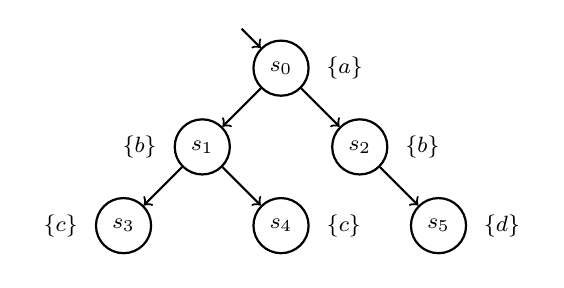
\begin{tikzpicture}[->,scale=1,label distance=0mm]
	\tikzstyle{every node}=[draw,shape=circle,minimum size=7mm,font=\footnotesize];
    \tikzstyle{every path}=[draw,thick];
    
    \node at (0, 0)  (s0) [label=right:${ \{a\} }$] {$s_0$};
    \node at (-1, -1) (s1) [label=left:${ \{b\} }$] {$s_1$};
    \node at (1, -1)  (s2) [label=right:${ \{b\} }$] {$s_2$};
    \node at (-2, -2)  (s3) [label=left:${ \{c\} }$] {$s_3$};
    \node at (0, -2)  (s4) [label=right:${ \{c\} }$] {$s_4$};
    \node at (2, -2)  (s5) [label=right:${ \{d\} }$] {$s_5$};

    \draw (-0.5, 0.5) to (s0);
    \draw (s0) to (s1);
    \draw (s0) to (s2);
	\draw (s1) to (s3);
	\draw (s1) to (s4);
    \draw (s2) to (s5);
\end{tikzpicture}
\end{center}

\begin{eqnarray*}
H_{0} &=&\{(s_{0},s_{0})\} \\
H_{1} &=&\{(s_{0},s_{0}),(s_{1},s_{1})\} \\
H_{2} &=&\{(s_{0},s_{0}),(s_{1},s_{1}),(s_{2},s_{2})\} \\
H_{3} &=&\{(s_{0},s_{0}),(s_{1},s_{1}),(s_{2},s_{2}),(s_{3},s_{3})\} \\
H_{4}
&=&\{(s_{0},s_{0}),(s_{1},s_{1}),(s_{2},s_{2}),(s_{3},s_{3}),(s_{4},s_{4})\}
\\
H_{5}
&=&%
\{(s_{0},s_{0}),(s_{1},s_{1}),(s_{2},s_{2}),(s_{3},s_{3}),(s_{4},s_{4}),(s_{5},s_{5})\}
\\
H_{6} &=&H_{5}
\end{eqnarray*}

\bigskip
